\lecture{2009-12-16}
\section{Reihen, Potenzreihen, Taylorreihen}

\subsection{Schneeflockenkurve nach Koch, Reihen}

Passend zu Weihnachten: Konstruktion einer Schneeflocke mit $\infty$-großem Umfang, aber endlicher Fläche

\subsubsection*{Konstruktion}
Start: gleichseitiges $\triangle s_1$ der Kantenlänge $1$: Fläche $F_1$, Umfang $U_1$

\begin{center}
    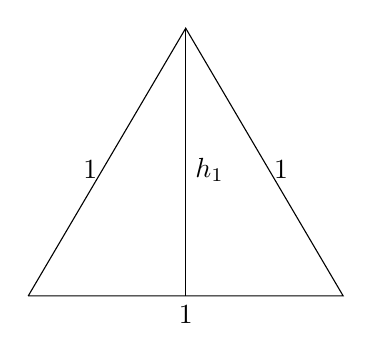
\begin{tikzpicture}[scale=1, x=1cm, y=1cm]
	    \draw (-2, 0) -- (2, 0) -- (0, 3.4) -- (-2, 0);
	    \draw (0, 0) -- (0, 3.4);
	    \draw (0, 1.6) node [right] {$h_1$};
	    \draw (1, 1.6) node [right] {$1$};
	    \draw (0, 0) node [below] {$1$};
	    \draw (-1, 1.6) node [left] {$1$};
    \end{tikzpicture}
\end{center}

\begin{align*}
    g_1 &= 1 \\
    h_1^2 + \left(\frac{1}{2}\right)^2 &= 1^2 \\
    F_{\triangle} &= \frac{g h}{2} \\
    \implies h_1 &= \frac{1}{2} \sqrt{3}
\end{align*}

zu $\triangle s_1$:
\begin{align*}
    U_1 &= 3 g_1 = 3 \\
    F_1 &= \frac{1}{4} \sqrt{3} \hspace{20px} \text{($g_1 h_1$: 2)}
\end{align*}

\subsubsection*{1. Schritt (Rekursion für alle Schritte):}

Drittle jede Seite und errichte über dem Mittelstück ein gleichseitiges $\triangle$

\begin{center}
    \begin{tikzpicture}[decoration=Koch snowflake, scale=1, x=1cm, y=1cm] % wtf tikz
        \draw decorate{(-2, 0) -- (0, 3.4) -- (2, 0) -- (-2, 0)};
    \end{tikzpicture}
\end{center}

\begin{align*}
    F_2 &= F_1 + 3 F_{\text{kl} \triangle} \\
    F_{\text{kl} \triangle} &= \frac{1}{2} \cdot g_2 \cdot h_2 \\
    &= \frac{1}{2} \cdot \frac{1}{3} \cdot h_2 \\
\\
    h_2^2 + \left( \frac{1}{6} \right)^2 &= \left( \frac{1}{3} \right)^2 \\
    \implies h_2 &= \frac{1}{3} \cdot \sqrt{ \frac{3}{4} } \\
\\
    \implies F_{\text{kl} \triangle} &= \frac{1}{9} \left( \frac{1}{4} \sqrt{3} \right)
\\
    U_2 &= U_1 + 3 \cdot g_2 = 4
\end{align*}

\subsubsection*{2. (allgemeiner) Schritt:}
Drittelung über alle Begrenzungsgeraden von $s_2$ liefert den 18-zackigen Stern $s_3$
%
\begin{center}
    \begin{tikzpicture}[decoration=Koch snowflake, scale=1, x=1cm, y=1cm]
		\draw decorate{ decorate{(-2, 0) -- (2, 0)} };
	\end{tikzpicture}
\end{center}
%
Konstruktionsprinzip: 3 Zacken werden vervierfacht
%
\begin{align*}
    F_3 &= F_2 + 3 \cdot 4 \cdot F_{\text{neu}} \\
    U_3 &= U_2 + 12 \cdot \frac{1}{9} \\
\\
    F_{\text{neu}} &= \frac{1}{2} \cdot h_3 \cdot g_3 \\
    &= \frac{1}{4} \cdot \sqrt{3} \cdot \frac{1}{9^2}
\end{align*}
%
allgemein ($n > 2$):
\begin{align*}
    F_n &= F_{n-1} + 3 \cdot 4^{n-2} \left( \frac{1}{4} \cdot \sqrt{3} \cdot \frac{1}{9^{n-1}} \right) \\
    U_n &= U_{n-1} + \left( \frac{4}{3} \right)^{n-2}
\end{align*}
%
Beweis: vollständige Induktion, Beweismittel sind bereits erläutert\\
Auflösen der 2-Term-Rekursion:

\begin{align*}
    F_n &= \frac{1}{4} \sqrt{3} \left( 1 + \frac{1}{3} + \frac{1}{9} \sum_{k=1}^{n-2} \left( \frac{4}{9} \right)^k \right) \\
    U_n &= 4 + \sum_{k=1}^{n-2} \left( \frac{4}{3} \right)^k
\end{align*}

\subsubsection*{Begriffe zu Reihen}

Idee: führe die Form $\ds\sum_{k=0}^{\infty} a_k$ auf Folgen zurück

\begin{definition}[Partialsumme] Zu jeder reellen Zahlenfolge $(a_n)_{n \in \mathbb{N}}$ heißt die Folge
\begin{equation*}
    s_n = \sum_{k=1}^n a_k = a_1 + \dots + a_n
\end{equation*}
die $n$-te Partialsumme der Reihe $\sum_{k=1}^{\infty} a_k$
\end{definition}

\noindent Grenzwert der Reihe $\equals$ Folgengrenzwert der Partialsummen
% noch zu leisten: Interpretation/Anwendung

\begin{definition}
Eine Reihe $\sum_{k=1}^{\infty} a_k$ heißt konvergent (divergent) falls die Folge der Partialsummen konvergent (divergent) ist.
\end{definition}

\noindent Für Konvergenz-/Divergenz-Untersuchungen haben wir \emph{nur} ein \emph{zentrales Werkzeug}: die geometrische Reihe.
\begin{equation*}
    \sum_{k=1}^{\infty} x^{k-1} = \sum_{k=0}^{\infty} x^k =
    \begin{cases}
        \frac{1}{1-x} & |x| < 1 \quad\text{Konvergenz}\\
        \infty & |x| \geq 1 \quad\text{Divergenz}
    \end{cases}
\end{equation*}

\begin{note}
  Die Formel für $|x| < 1$ ergibt sich aus der allgemeinen Summenformel für die geometrische Reihe:
  \[ \liminfty{\sum_{k=0}^{n} x^k} = \liminfty{ \frac{1-x^{n+1}}{1-x}} = \frac{1}{1-x} \]
\end{note}


\subsubsection*{Anwendung: Schneeflockenkurve}
\begin{align*}
    F_n: x &= \frac{4}{9} \le 1 \implies \text{Konvergenz, endliche Fläche} \\
    U_n: x &= \frac{4}{3} \ge 1 \implies \text{Divergenz, unendliche Fläche}
\end{align*}

\subsubsection*{Intuitive Kriterien}

\begin{enumerate}
    \item Notwendig für Konvergenz der Reihe: Folgenelemente $(a_n)_{n \in \mathbb{N}}$ bilden eine \emph{Nullfolge}
    \item umgekehrter Schluss: $(a_n)_{n \in \mathbb{N}}$ Nullfolge $\not\Rightarrow$ Konvergenz der Reihe\\
        Gegenbeispiel: $\sum_{k=1}^{\infty} \frac{1}{k} \rightarrow \infty $ (siehe frühere Zweier-Potenzen) \\
        harmonische Reihe ist divergent
\end{enumerate}

\begin{note}
    "`$(a_n)_{n \in \mathbb{N}}$ Nullfolge"' ist \emph{notwendig}, aber nicht \emph{hinreichend}.
\end{note}

\begin{example} Die harmonische Reihe
  \[ \sum_{k=1}^{\infty} \frac{1}{k} \]
  divergiert, obwohl
  \[ a_k = \frac{1}{k} \] eine Nullfolge ist.
\end{example}

\begin{note} Allerdings ist
    \[ \epsilon > 0: \quad \sum_{k=1}^{\infty} \frac{1}{k^{1+\epsilon}} \]
    konvergent.
\end{note}

\subsubsection*{Rechenregeln für konvergente Reihenelemente}
\begin{enumerate}
    \item \begin{equation*} a = \sum_{k=1}^{\infty} a_k,\; b = \sum_{k=1}^{\infty} b_k \end{equation*}
        \begin{equation*}\implies \sum_{k = 1}^{\infty} \left( a_k \pm b_k \right) = \sum_{k=1}^{\infty} a_k \pm \sum_{k=1}^{\infty} b_k = a \pm b
        \end{equation*}
    \item \begin{equation*}c \in \mathbb{R} \implies \sum_{k=1}^{\infty} c a_k = c \cdot\sum_{k=1}^{\infty} a_k = c \cdot a \end{equation*}
    \item \begin{equation*}a_k \leq b_k \implies \sum_{k=1}^{\infty} a_k \leq \sum_{k=1}^{\infty} b_k \end{equation*}
\end{enumerate}

%\subsection{Konvergenzkriterien}

% Ausführungen in die nächste Vorlesung migriert -- LH
